% Options for packages loaded elsewhere
\PassOptionsToPackage{unicode}{hyperref}
\PassOptionsToPackage{hyphens}{url}
%
\documentclass[
]{article}
\title{NHL Realignment Effects on Playoff Qualification}
\author{Kilbourne Charrier, Michael Bauers, Clinton Rothschild, Sam
Downs}
\date{}

\usepackage{amsmath,amssymb}
\usepackage{lmodern}
\usepackage{iftex}
\ifPDFTeX
  \usepackage[T1]{fontenc}
  \usepackage[utf8]{inputenc}
  \usepackage{textcomp} % provide euro and other symbols
\else % if luatex or xetex
  \usepackage{unicode-math}
  \defaultfontfeatures{Scale=MatchLowercase}
  \defaultfontfeatures[\rmfamily]{Ligatures=TeX,Scale=1}
\fi
% Use upquote if available, for straight quotes in verbatim environments
\IfFileExists{upquote.sty}{\usepackage{upquote}}{}
\IfFileExists{microtype.sty}{% use microtype if available
  \usepackage[]{microtype}
  \UseMicrotypeSet[protrusion]{basicmath} % disable protrusion for tt fonts
}{}
\makeatletter
\@ifundefined{KOMAClassName}{% if non-KOMA class
  \IfFileExists{parskip.sty}{%
    \usepackage{parskip}
  }{% else
    \setlength{\parindent}{0pt}
    \setlength{\parskip}{6pt plus 2pt minus 1pt}}
}{% if KOMA class
  \KOMAoptions{parskip=half}}
\makeatother
\usepackage{xcolor}
\IfFileExists{xurl.sty}{\usepackage{xurl}}{} % add URL line breaks if available
\IfFileExists{bookmark.sty}{\usepackage{bookmark}}{\usepackage{hyperref}}
\hypersetup{
  pdftitle={NHL Realignment Effects on Playoff Qualification},
  pdfauthor={Kilbourne Charrier, Michael Bauers, Clinton Rothschild, Sam Downs},
  hidelinks,
  pdfcreator={LaTeX via pandoc}}
\urlstyle{same} % disable monospaced font for URLs
\usepackage[margin=1in]{geometry}
\usepackage{graphicx}
\makeatletter
\def\maxwidth{\ifdim\Gin@nat@width>\linewidth\linewidth\else\Gin@nat@width\fi}
\def\maxheight{\ifdim\Gin@nat@height>\textheight\textheight\else\Gin@nat@height\fi}
\makeatother
% Scale images if necessary, so that they will not overflow the page
% margins by default, and it is still possible to overwrite the defaults
% using explicit options in \includegraphics[width, height, ...]{}
\setkeys{Gin}{width=\maxwidth,height=\maxheight,keepaspectratio}
% Set default figure placement to htbp
\makeatletter
\def\fps@figure{htbp}
\makeatother
\setlength{\emergencystretch}{3em} % prevent overfull lines
\providecommand{\tightlist}{%
  \setlength{\itemsep}{0pt}\setlength{\parskip}{0pt}}
\setcounter{secnumdepth}{-\maxdimen} % remove section numbering
\ifLuaTeX
  \usepackage{selnolig}  % disable illegal ligatures
\fi

\begin{document}
\maketitle

\hypertarget{motivation}{%
\section{Motivation}\label{motivation}}

In the 2013-14 National Hockey League (NHL) season, the league made some
changes to the conference numbers. The Winnipeg Jets moved from the
Eastern conference to the Western conference. This created an imbalance
in the conference numbers giving the Eastern conference sixteen teams
and leaving the Western conference with only fourteen teams. From the
start, it already seemed unfair to have more teams in one conference
than the other. If every team had equal skill, the fourteen teams in the
western conference had an equal one four in seven chance of making it to
the playoffs. In contrast, the sixteen teams in the eastern conference
had a fifty percent chance of making it to the playoffs. This uneven
probabillity will be known for the rest of the paper as the conference
gap.

Now how could an organization as big as the NHL allow for that kind of
discrepency between the conferences? As a continuation of our research
we wanted to look at another season with a similiar balance shift in the
conferences to see how that change could have affected the outcome of
the season. The season we chose was the recent expansion draft season of
2017-18. Before the start of the season, the NHL added a new franchise
in the Las Vegas Golden Knights. This team was set to join the Western
conference. This shifted the conference split from fourteen to sixtten
West to East to a closer fifteen to sixteen split. We wanted to see if
our result was statistically significant from both the conference gap of
an even season and the conference gap from our tested 2013-14 season.

\hypertarget{introduction}{%
\subsection{Introduction}\label{introduction}}

In 2011 the Atlanta Thrashers became the Winnipeg Jets. A problem was
presented as Winnipeg is considerably far from the east coast of the
North American continent. Because of this and how the season is set up,
the average travel time for teams playing winnipeg were fairly large as
eastern conference teams play each other more often. Just before the
start of the 2013-14 season, the league offices for the NHL decided to
move over the Winnipeg Jets from the Eastern conference to the Western
conference and in return the Eastern conference aquired the Columbus
Blue Jackets and the Detroit Redwings. This left the the two conferences
at an uneven balance. The Eastern conference now had sixteen teams while
the Western conference only had fourteen teams. This presented a curious
problem as for both conferences, eight teams make the playoff brackets.
It is easy to see the problem at hand that the western conference has
just as many playoff slots for having two fewer teams. The goal of our
analysis and the paper we based our ideas off of and partially
replicated, was to discover what that difference could mean in the
greater sense of the league moving forward with this set up. We did this
based on the average points and wins necessary to make the playoffs for
both conferences.

To further our study, we also looked at the 2017-18 season. This season
is important because it gave the introduction of a new team in the
league known as the Vegas Golden Knights. This team was introduced into
the Pacific division of the Western conference, this meant that the
balance between the number of teams in the East and West was more equal
than the 2013-2014 split. Our goal for this was to investigate how this
new conference structure could affect the conference gap. We used the
same process to investigate this new season's structure as our previous
analysis of the 2013-14 season. Given that the difference in the number
of teams between conferences is less severe we suspected that our
estimated conference gap under this setup (3 Divisions of 8 teams, 1
Division of 7 teams) would lie somewhere around the halfway point
between the estimate for the pre 2013-2014 structure (6 Divisions of 5
teams each) and the 2013-2014 season (2 Divisions of 8 teams, 2
Divisions of 7 teams).

\hypertarget{pre-2013-2014-nhl-conference-structure}{%
\subsection{Pre 2013-2014 NHL Conference
Structure}\label{pre-2013-2014-nhl-conference-structure}}

\includegraphics[width=0.6\textwidth,height=\textheight]{Images/pre2013struct.png}

\hypertarget{nhl-conference-structure}{%
\subsection{2013-2014 NHL Conference
Structure}\label{nhl-conference-structure}}

\includegraphics[width=0.6\textwidth,height=\textheight]{Images/2013struct.png}

\hypertarget{nhl-conference-structure-1}{%
\subsection{2017-2018 NHL Conference
Structure}\label{nhl-conference-structure-1}}

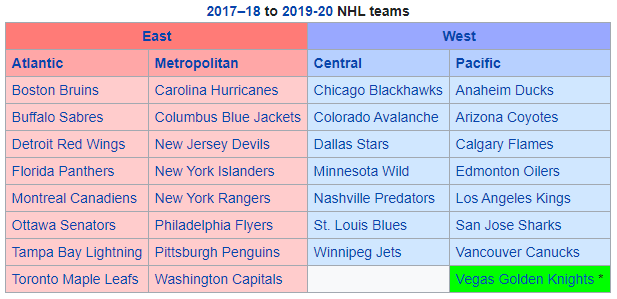
\includegraphics[width=0.6\textwidth,height=\textheight]{Images/2017struct.png}

\hypertarget{methodology}{%
\section{Methodology}\label{methodology}}

\hypertarget{basic-idea}{%
\subsection{Basic Idea}\label{basic-idea}}

The basic idea behind the model is that all of the teams have a base
``skill level'' that they play at or near during any given game
throughout the season. Each game is competitive because we aren't sure
how well either team will play, and even a team with a higher skill
level can be beaten by another team for any number of reasons. We keep
track of this skill level and draw other metrics based off of it, then
use the metrics to compute a team's score for the season. This score is
used to calculate the team's seed in their respective conference and
division.

\hypertarget{creating-the-model}{%
\subsection{Creating the Model}\label{creating-the-model}}

To start out, we first need to make sure that we calculate the
game-to-game performance levels given by \(\tau\) and the standard
deviation of the team's talent levels given by \(\sigma\). These are
related to the following ratio, where p is the probability that the
worst team in the league beats the best team in the league.

\(-\frac{2.8854}{\Phi^{-1}(p)} = \frac{\tau}{\sigma}\)

Based on the data from all of the seasons with 30 teams, we can
calculate that the team with the worst record in the league beat the
team with the best team about a quarter of the time. We choose to set p
equal to 0.25 for this reason, making the ratio \(\tau/\sigma\) = 4.28.
This means that there are four times the variability in the team's
performances in game than there is in the talent levels of the teams.
The actual values of \(\tau\) and \(\sigma\) don't matter, just the
ratio, but for simplicity we will set \(\tau\) equal to 4.28 and
\(\sigma\) equal to 1.

We then want to simulate a skill level metric for each of the thirty
teams. We create the metric from the following distribution, with team i
being equal to \(\mu_{i}\).

\(\mu_{i}\)\textasciitilde{}\(N(0,\sigma^{2})\)

We draw the values from a normal distribution because in sports the
overall performace of the teams is generally normally distributed. That
is, there are a few really good teams, a few really bad teams, and a lot
of teams in between.

We hold the team skill levels constant throughout the season, this make
intuitive sense, because there are very seldom large changes to the
team's rosters or strategies throughout a season, but after each season
teams often make at least some change.

When drawing the season schedule for each simulation we chose just to
use the same schedule as the real world NHL for that year. If we had
taken into account some sort of measure of the performance of real world
teams into our model this may have influenced the results to our
research question. However since team skill is a random variable drawn
at the start of each simulation with no relation to the real world skill
of these teams this should not bias our results.

For each game that is played in the season we draw a performance metric
for both competing teams. This metric is drawn from a normal
distribution with the mean being equal to the team's skill level and the
standard deviation being equal to \(\tau^{2}\). This is based on the
idea that a team with any skill level will play somewhere around their
skill level, rarely playing much worse and rarely playing much better.
This metric is calculated as such, with i indicating the home team and j
indicating the away team.

\(\gamma_{i}\)\textasciitilde{}\(N(\mu_{i}, \tau^{2})\)

\(\gamma_{j}\)\textasciitilde{}\(N(\mu_{j}, \tau^{2})\)

Logically, the winner of each game would be decided by the higher value
of \(\gamma\), but in hockey it is possible for the game to go into
overtime. This happens in about 22.4\% of the games that were played
over the past 15 seasons, so we must solve the following equasion for
\(\alpha\):

\(Pr(|\gamma_{i}-\gamma_{j}| < \alpha) = 22.4\)\%

Solving this equasion gives us a value of \(\alpha \approx 1.769.\)

If there is a game in which \(|\gamma_{i}-\gamma_{j}|\geq \alpha\), the
team with the higher \(\gamma\) value is awarded a win and is therefore
given two points while the team with the lower \(\gamma\) value is given
0 points. For games in which \(|\gamma_{i}-\gamma_{j}| < \alpha\), the
game is considered a tie.

In the case of a tie we linearly resale the \(\gamma\) values with the
following formula:

\(\zeta = \frac{(\gamma_{i}-\gamma_{j}) - a}{b}\)

Where a is the mean and b is the maximum of all
\(\gamma_{i}-\gamma_{j}\) values from that season.

Using the resulting value of \(\zeta\) we use a Bernoulli distribution
to simulate a weighted coin flip, with a success meaning that the home
team wins and a failure meaning the away team wins.

Winner \textasciitilde{} \(Bernoulli(\zeta_{ij})\)

The winning team receives two points while the losing team receives one
point.

For each team the sum of points accumulated over the season was taken
and teams were then sorted into conference and division. The
qualifications for making the playoffs under each of our 3 seasons were
then applied to the point totals for teams to determine seeding.
Conference gap was then calculated by finding the difference in points
between the 8th seed in the West and the 8th seed in the East. This
process represents simulating a single season.

We simulated 10,000 seasons for both the 2013-2014 and 2017-2018
analysis. We then calculate the conference gap for both the old and the
new ruleset as the average conference gap across all simulations. We
also save the number of points earned by each seed to do analysis on
later.

\hypertarget{additional-model-details}{%
\subsection{Additional model details}\label{additional-model-details}}

Our model does not account for the real-world skill of teams, but
because we are not doing any inference on specific team performance
depending on rule changes this is not relevant. Because we are
interested in the difference in scores of the 8th seeds we actually
don't even need any real-world teams and can instead replace them with
placeholders or just numbers. The lack of a need for real world data was
also an advantage to our analysis as it meant our results may be
expressed as a general representation of the ``fairness'' of these
conference structures since they are not related to the skill of real
world teams.

An alternative choice we could have made is that in the event of a tie
we could have given either team a 50\% chance of winning instead of
linearly rescaling the values and using a weighted coin flip, but we
don't know exactly how the outcome of NHL overtime games usually end up
skewing -- whether it be in favor of the better team or if it is
distributed more randomly.

When performing analysis on the 2017-2018 conference structure we chose
to hold our parameters \(p,\tau\) and \(\sigma\) to be the same as
stated above in the 2013-2014 analysis since we are talking about a
reasonable small amount of time passing between these two seasons we
thought it would be unreasonable to think that they would alter all that
much. The same number of simulations were run also to make results more
easily comparable.

\hypertarget{results}{%
\section{Results}\label{results}}

After doing 10,000 simulations of full NHL seasons using the Monte Carlo
simulation methods detailed above, the results can be seen in the
figures below. The red shaded graph represents the gap between the East
and West 8th seeds (conference gap) under the conference and division
alignment in the 2013-14 NHL season while the blue graph represents the
gap between the East and West 8th seeds (conference gap) under the
conference and division alignment in the 2012-2013 NHL season. The mean
conference gap for the new alignment (2013-2014) is 2.30 points while
the mean conference gap for the old alignment (2012-2013) is practically
zero at -0.02 points.

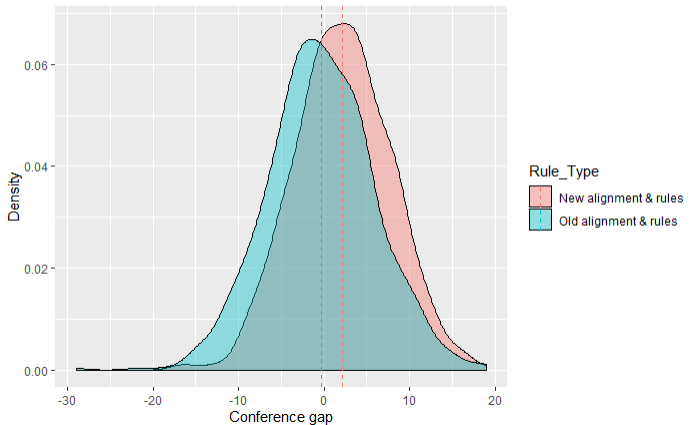
\includegraphics[width=0.85\textwidth,height=\textheight]{Images/GapVis.png}

When looking at the 2017-2018 season we can see something close to what
we hypothesized in our introduction, our conference gap does indeed lie
somewhat close to halfway between the estimate for the 2013-2014 season
and 2012-2013. When rerunning the analysis for 2017-2018 our estimate
for conference gap under the 2012-2013 structure was 0.038 which is
close to what was estimated above and makes sense as we expect the
conferences to be equal in terms of likliehood of making the playoffs
under these rules. The mean conference gap across our simulations for
the 2017-2018 season was 1.091 which is approximately halfway between 0
and 2.3. It should be noticed that visually it can be seen that the
density for the 2017-2018 season conference gap more closesly resembles
the 2012-2013 density than the 2013-2014 density did.

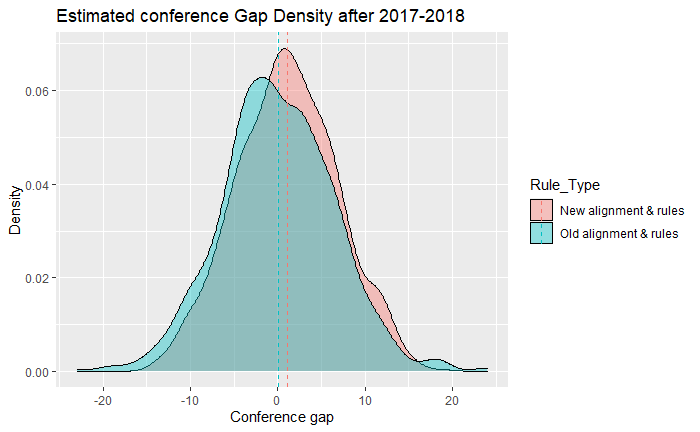
\includegraphics[width=0.85\textwidth,height=\textheight]{Images/gapvis20172018.png}

Looking at these results, the numbers fall in line with what would be
the logical expectation under these circumstances. The 2013-2014
structure moves the balance of teams over towards the East with 16 teams
while the West sits at 14 teams. With more teams in the East, it makes
sense that the East would have more teams with higher number of total
points from the season. To look at these results in a different light,
it is key to translate these numbers to the point scoring system of the
NHL. On average, the difference between the conference gaps of the two
division alignments (2012-2013,2013-2014) comes out to be 2.32 in favor
of the 2013-2014 alignment/structure. Under the 2017-2018 analyis our
difference in conference gap between alignments comes out to be 1.053
(1.091-0.038). This result makes sense since the conferences are still
unbalanced with the East having more teams than the West (16 and 15
respectively) but less unbalanced than 2013-2014 (16 and 14
respectively) The conference gap has been calculated as:

East 8th Seed Season Total Points - West 8th Seed Season Total Points

The mean conference gap, in terms of total points, means that the East's
8th seeded team has on average 2.30 more points than the West's 8th
seeded team for 2013-2014, similarly we expect the 8th seed in the
Eastern conference to have 1.091 more points than their Western
conference counterpart under the 2017-2018 structure. In the NHL, a team
earns 2 points for a win, 1 point for an overtime loss, and 0 points for
a loss. With this point system,under the 2013-2014 alignment the East's
8th seeded team on average needs to win one more game during the season
or exchange two losses for two losses in overtime. This favors Western
conference teams in the way they have to earn less total points
throughout the season to make the playoffs than Eastern conference
teams. This same bias towards Western conference teams to make the
playoffs is present under the 2017-2018 bias but the practical effects
of a one point difference is not even worth a single win in an 82 game
season, so although this effect is present it's not as drastic.

Not only were the 8th seeds from each conference calculated but each
seed for the whole NHL. These box and whisker plots show a wide range of
information for the total points for each seed across the 10,000
simulated seasons for both the 2013-2014 and 2017-2018 alignemnts. The
endpoints of the whiskers represent the outlier point totals earned by
each seed. The sides of the box represent the 2.5\% and 97.5\%
quantiles. The line within the box represents the mean. The structure of
this plot makes sense with the curve of less points the lower seed and
more points the higher seed the team achieves. The higher the number on
the x axis the lower seed of the team; 30 being the worst team in the
league (31 for 2017-2018 simulation) and 1 being the best team in the
league. Interesting feautures of these plots are a tight spread of
simulated points for teams seeded around the middle of the league. This
makes sense given that these point values are probably closer to the
mean point total for a season and thus more likely under the model we
defined. Another note is that the overall range of point totals is
greater in the 2013-2014 simulation than it is under the 2017-2018
simulation. This has been compared with real NHL data and the shape
lines up in a similar fashion.

\hypertarget{points-by-seed}{%
\subsection{2013-2014 Points by Seed}\label{points-by-seed}}

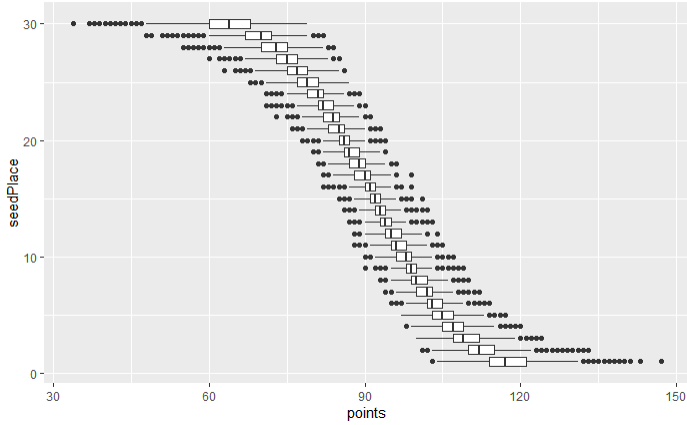
\includegraphics[width=0.8\textwidth,height=\textheight]{Images/SeedPlace.png}

\hypertarget{points-by-seed-1}{%
\subsection{2017-2018 Points by Seed}\label{points-by-seed-1}}

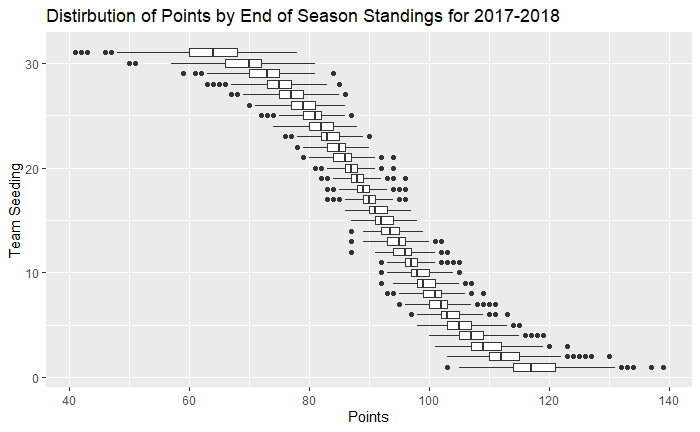
\includegraphics[width=0.8\textwidth,height=\textheight]{Images/seedplace20172018.png}

\hypertarget{conclusion}{%
\section{Conclusion}\label{conclusion}}

Since the change to the conference structure of the NHL to be
unbalanced, there have been questions on whether these structures are
giving an unfair advantage for one of the conferences: more specifically
the Western Conference. With the West having two less teams under the
2013-2014 alignment, it was inferred that each of those teams would have
a better chance of making the playoffs. They wouldn't need to earn as
many points to secure a playoff spot as teams in the Eastern Conference.
After running 10,000 Monte Carlo simulations of the 2013-2014 NHL
season, the results support the case that the Western Conference has a
noticeable advantage over the Eastern Conference. The 8th seed in the
east on average has an end of season point total of 2.3 (1.091 for
2017-2018) points higher than the 8th seed in the west. This can cause
problems because a statistically worse team can make the playoffs in the
Western Conference while a better team might miss out in the Eastern
Conference. This is support of the idea that these rules introduce a
bias agaisnt teams in the Eastern conference which goes agaisnt the
league being ``fair'' to all teams.

\hypertarget{references}{%
\section{References}\label{references}}

\begin{itemize}
\item
  Pettigrew, Stephen. ``How the West Will Be Won: Using Monte Carlo
  Simulations to Estimate the Effects of NHL Realignment.'' Journal of
  Quantitative Analysis in Sports, vol.~10, no. 3, 1 Jan.~2014,
  10.1515/jqas-2013-0125. Accessed 10 Dec.~2020.
\item
  History of Organizational Changes in the NHL. 26 Nov.~2020,
  en.wikipedia.org/wiki/History\_of\_organizational\_changes\_in\_the\_NHL.
  Accessed 10 Dec.~2020.
\end{itemize}

\end{document}
